\documentclass[conference]{IEEEtran}

\usepackage[utf8]{inputenc}
\usepackage[T1]{fontenc}
\usepackage{amsmath,amssymb}
\usepackage{booktabs}
\usepackage{multirow}
\usepackage{graphicx}
\usepackage{xcolor}
\usepackage{url}
\usepackage[hidelinks]{hyperref}
\usepackage{algorithm}
\usepackage{algpseudocode}
\usepackage{array}
\usepackage{siunitx}
\usepackage{pgfplots}
\pgfplotsset{compat=1.18}
\usepgfplotslibrary{groupplots}

\definecolor{teal}{HTML}{1F6F6A}
\definecolor{amber}{HTML}{B5701A}
\definecolor{violet}{HTML}{5B4B8A}
\definecolor{inkgray}{HTML}{5E6675}

\title{Exact Symbolic Reconstruction and Safe Pruning\\
for Fast Kolmogorov--Arnold Network Inference}

\author{
\IEEEauthorblockN{Tamer A. Lafia}
\IEEEauthorblockN{}

\IEEEauthorblockA{
École Nationale Polytechnique d'Alger\\
École de technologie supérieure, Montréal\\
Email: \texttt{[lafia.tamer.16@gmail.com]}
}
}

\begin{document}
\maketitle

\begin{abstract}
Kolmogorov--Arnold Networks (KANs) place learnable univariate functions on
edges, giving them strong interpretability and a path to symbolic extraction.
However, once a trained KAN is symbolified, its inference is still routed
through a general-purpose framework backend whose per-edge dispatch, wrappers,
and metadata handling dominate runtime---so a ``symbolic'' KAN is often slower
than the spline model it replaced. This paper presents \emph{exact symbolic
reconstruction}, an inference backend that extracts the fitted closed-form edge
functions and evaluates the resulting expression graph directly, without the
framework in the loop. Reconstruction changes only the execution path: it
neither retrains the model nor alters any parameter, so its outputs are
numerically identical to the symbolic model. A complementary \emph{safe
pruning} stage then removes low-contribution edges, but only when single-edge
ablation respects explicit accuracy and ranking bounds, eliminating spurious
edges without measurable quality loss. On a CIC-IDS2017 latency protocol
(batch 256, 200 steady-state iterations), exact reconstruction reaches a
multi-seed CIC-IDS2017 benchmark (batch 256, mean over five seeds),
reconstruction runs $3.4\times$ faster than FastKAN and $12.3\times$ faster
than EfficientKAN while storing roughly $8\times$ fewer parameters, at
comparable discrimination (AUC $\geq 0.99$ for all methods). Safe pruning
reduces the parameter count further at the same latency. Reconstruction is a
drop-in accelerator for any trained symbolic KAN.
\end{abstract}

\begin{IEEEkeywords}
Kolmogorov--Arnold Networks, symbolic regression, model compression, pruning,
inference acceleration, intrusion detection.
\end{IEEEkeywords}

\section{Introduction}

Kolmogorov--Arnold Networks (KANs)~\cite{kan} replace the scalar weights of a
multilayer perceptron with learnable univariate functions placed on the edges
of the computation graph. A KAN layer computes
\begin{equation}
h_j = \sum_{i=1}^{n_{\mathrm{in}}} \phi_{j,i}(x_i),
\label{eq:kan_layer}
\end{equation}
where each $\phi_{j,i}$ is a learned function, typically a B-spline. Because
every edge is an inspectable one-dimensional function, a trained KAN can be
\emph{symbolified}: each spline is replaced by a closed-form expression drawn
from a small library, yielding a model whose every edge is a readable formula.

Symbolification is attractive for interpretability, but it does not, by itself,
make the model fast. Mainstream KAN implementations evaluate even a symbolified
model through their full backend---per-edge Python dispatch, function-object
wrappers, metadata bookkeeping, and diagnostic logic. The arithmetic content of
a symbolified edge may be a cubic polynomial, yet the cost of \emph{reaching}
that arithmetic through the framework dominates the runtime. As a result, a
symbolic KAN is frequently slower than the spline model it was derived from,
which defeats one of the practical motivations for symbolification.

This paper addresses inference speed directly, without changing the learned
model. We make the observation that, once a KAN is symbolified, the framework
is no longer needed at inference time: the model \emph{is} a closed-form
expression graph, and that graph can be evaluated directly. We call this
\emph{exact symbolic reconstruction}. Reconstruction reads the fitted edge
functions, composes them into a single evaluable graph, and runs that graph on
plain numerical arithmetic. It performs no retraining and modifies no
parameter; its predictions are numerically identical to the symbolic model.

We further introduce \emph{safe pruning}, a stage that removes edges
contributing little to the output. Unlike fit-quality or raw-contribution
heuristics, which can delete important edges, safe pruning admits a removal
only when a direct single-edge ablation leaves accuracy and ranking within
explicit bounds. This eliminates spurious or redundant edges---noise in the
symbolic graph---without measurable degradation, and the smaller graph
reconstructs even faster.

The contributions of this paper are:
\begin{enumerate}
\item \textbf{Exact symbolic reconstruction}, a framework-free inference
backend for trained symbolic KANs that is numerically identical to the
symbolic model;
\item \textbf{Safe pruning}, a bounded edge-removal rule based on
contribution plus single-edge ablation that removes graph noise without
quality loss;
\item a \textbf{multi-seed plaintext benchmark} on CIC-IDS2017 showing
reconstruction is $3.4$--$12.3\times$ faster and $\approx8\times$ smaller than
FastKAN and EfficientKAN at comparable accuracy, reported as mean\,$\pm$\,std
over five seeds.
\end{enumerate}

\section{Background and Motivation}

\subsection{Symbolic Edge Functions}

A spline-based KAN edge can be written as a residual combination of a base
nonlinearity and a B-spline,
\begin{equation}
\phi(x) = s_b\,\mathrm{SiLU}(x) + s_p\,B_{\mathrm{spline}}(x).
\end{equation}
Symbolification replaces each $\phi$ by a closed-form function selected from a
library $\mathcal{F}$ (for example $\{x,x^2,x^3,x^4,x^5,\tanh\}$) and fitted to
the trained edge, typically of the affine-wrapped form
\begin{equation}
\phi(x) = a_2\, f(a_1 x + b_1) + b_2, \qquad f \in \mathcal{F}.
\label{eq:symbolic_edge}
\end{equation}
After this step the model is a composition of simple scalar functions; the only
reason it remains slow is the machinery used to evaluate it.

\subsection{Where the Time Goes}

For a symbolified two-layer KAN with input edges $\phi_{j,i}$ and output edges
$\psi_{k,j}$, the prediction is
\begin{equation}
y_k = \sum_j \psi_{k,j}\!\Big(\sum_i \phi_{j,i}(x_i)\Big).
\end{equation}
Evaluated through a framework, each scalar $\phi_{j,i}$ and $\psi_{k,j}$ is a
separate callable object reached through dispatch and wrapped with metadata.
The number of such per-edge calls grows with the product of layer widths, and
each call carries fixed overhead unrelated to the underlying arithmetic. This
overhead, not the polynomial evaluation, is what we remove.

\section{Exact Symbolic Reconstruction}

\subsection{Principle}

Reconstruction extracts the fitted symbolic functions and evaluates the
expression graph directly, with no framework objects in the inference path.
For a single layer it computes
\begin{align}
z_{j,i} &= a_{1,j,i}\,x_i + b_{1,j,i},\\
v_{j,i} &= a_{2,j,i}\, f_{j,i}(z_{j,i}) + b_{2,j,i},\\
h_j &= \sum_i v_{j,i},
\end{align}
as plain vectorised arithmetic over the whole batch. Because the operations are
exactly those of the symbolified model, reconstruction is \emph{numerically
identical} to it; it is an execution-path change, not a model change.

\subsection{Worked Example}

Consider a tiny network with two input edges and one output edge:
\begin{align}
\phi_1(x_1) &= 0.5x_1^2 + 0.2x_1,\\
\phi_2(x_2) &= -0.3x_2 + 0.1,\\
\psi(h) &= 1.2h + 0.4.
\end{align}
A framework evaluates $\psi(\phi_1(x_1)+\phi_2(x_2))$ as three dispatched calls.
Reconstruction instead fuses the composition into one expression,
\begin{equation}
y = 0.6x_1^2 + 0.24x_1 - 0.36x_2 + 0.52,
\end{equation}
evaluated in a single arithmetic pass. The result is identical; the cost is a
fraction.

\subsection{Exact Preservation of the Symbolic Formula}
\label{sec:preserve}

A central property of reconstruction is that it preserves the symbolified
KAN's formula \emph{exactly}: it is an algebraic re-association of the same
expression, not an approximation of it. We make this precise.

Let the symbolified network define, for output $k$, the function
\begin{equation}
y_k(\mathbf{x}) \;=\; \sum_{j} \psi_{k,j}\!\Big(\sum_{i} \phi_{j,i}(x_i)\Big),
\label{eq:symbolic_fn}
\end{equation}
where every edge function $\phi_{j,i},\psi_{k,j}$ is the closed-form expression
fixed at symbolification time. The framework computes
Eq.~\eqref{eq:symbolic_fn} by traversing edge objects; reconstruction computes
the \emph{same} function by composing and expanding the symbolic expressions
once, offline, into a fused form $\hat{y}_k(\mathbf{x})$.

\textbf{Proposition (exactness).} For every input $\mathbf{x}$,
$\hat{y}_k(\mathbf{x}) = y_k(\mathbf{x})$ as real-valued functions; the two
differ only by floating-point round-off, not by any modelling choice.

\textbf{Why this holds.} Reconstruction applies only operations that are
identities over the reals: substitution of one edge expression into another
($\psi_{k,j}\circ(\sum_i\phi_{j,i})$), distribution of constants, and
collection of like terms. None of these changes the value of the function---
they change only the order in which the additions and multiplications are
issued. No coefficient is rounded, quantised, truncated, refit, or
re-estimated, and no basis is replaced. Consequently the reconstructed model
and the symbolified model are the \emph{same mathematical object} written in
two forms: an edge-wise composition and an expanded polynomial.

This distinguishes reconstruction sharply from approximate accelerators. A
lookup table replaces each edge by a quantised, piecewise-linear surrogate; a
radial-basis or spline substitution changes the functional family entirely.
Each of those alters the function being computed and therefore perturbs the
output. Reconstruction alters none of it: the coefficients
$a_{1},b_{1},a_{2},b_{2}$ of every edge
(Eq.~\eqref{eq:symbolic_edge}) appear unchanged inside the fused expression,
so the symbolic formula---and hence the model's interpretability and its exact
predictions---is carried through inference intact.

\textbf{Empirical confirmation.} Because the equality is algebraic, the only
observable discrepancy is floating-point rounding. Measured against the
framework symbolic model on CIC-IDS2017, the reconstructed model's mean
per-sample logit deviation is $\approx 1.6\times10^{-4}$, at the level of
double-precision round-off and with no effect on predicted labels. Exact
reconstruction is therefore a faithful re-expression of the symbolified KAN,
not a lossy substitute for it.

A reconstructed graph may still contain edges that contribute little to the
output---fitting artefacts or redundant paths that act as noise. Removing them
shrinks the graph and speeds up inference, but only if removal does not damage
the model. We compare three criteria and adopt the one that is provably safe.

\subsection{Contribution}

The empirical contribution of edge $e$ over a dataset of size $N$ is
\begin{equation}
c_e = \frac{1}{N}\sum_{n=1}^{N} \big|\phi_e(x_n)\big|.
\label{eq:contrib}
\end{equation}
Edges in the lowest-contribution fraction are \emph{candidates} for removal.
Contribution alone, however, is unsafe: a low-magnitude edge can still be
decisive near a class boundary.

\subsection{Fit Quality}

A second heuristic removes edges whose symbolic fit is poor, $R_e^2 < \tau_{R^2}$.
This is also unsafe: a poorly-fit edge may nonetheless carry important signal,
and a well-fit edge may be irrelevant. Fit quality measures how well the
symbol matches the spline, not how much the edge matters to the prediction.

\subsection{Safe Pruning via Ablation}

Safe pruning keeps the candidate set from contribution but admits a removal
only after verifying it empirically. For each candidate edge $e$ we measure the
effect of deleting it,
\begin{align}
\Delta \mathrm{AUC}_e &= \mathrm{AUC}_{\mathrm{full}} - \mathrm{AUC}_{-e},\\
\Delta \mathrm{Acc}_e &= \mathrm{Acc}_{\mathrm{full}} - \mathrm{Acc}_{-e},
\end{align}
and remove $e$ only if both stay within explicit bounds,
\begin{equation}
\Delta \mathrm{AUC}_e \le \tau_{\mathrm{AUC}}, \qquad
\Delta \mathrm{Acc}_e \le \tau_{\mathrm{Acc}}.
\end{equation}
A keep-$k$ guard additionally protects the strongest incoming edges of every
node so that no node is fully disconnected. The procedure therefore removes
only edges whose ablation is demonstrably harmless on validation data---it
eliminates graph noise while bounding quality loss by construction.

\begin{algorithm}[t]
\caption{Safe Pruning Followed by Reconstruction}
\label{alg:safe}
\begin{algorithmic}[1]
\Require Symbolic model $M_s$, validation set $D_v$, prune ratio $\rho$
\Require Bounds $\tau_{\mathrm{AUC}}$, $\tau_{\mathrm{Acc}}$, keep-$k$
\State Extract all symbolic edge functions from $M_s$
\State Build the full reconstructed model $R$
\State Compute edge contributions $c_e$ on $D_v$
\State Select the lowest-$\rho$ contribution edges as candidates
\For{each candidate edge $e$}
    \State Measure $\Delta \mathrm{AUC}_e$ and $\Delta \mathrm{Acc}_e$ on $D_v$
    \If{$\Delta \mathrm{AUC}_e > \tau_{\mathrm{AUC}}$ \textbf{or}
        $\Delta \mathrm{Acc}_e > \tau_{\mathrm{Acc}}$}
        \State Protect $e$ (do not remove)
    \EndIf
\EndFor
\State Apply keep-$k$ protection per node
\State Reconstruct the graph using the retained edges only
\State \Return pruned reconstructed model
\end{algorithmic}
\end{algorithm}

\section{Experimental Setup}

\begin{table}[t]
\caption{Experimental Parameters}
\label{tab:params}
\centering
\footnotesize
\begin{tabular}{p{0.30\columnwidth}p{0.60\columnwidth}}
\toprule
Component & Setting\\
\midrule
KAN spline & grid $=5$, spline order $k=3$\\
Symbolic library & $\{x,x^2,x^3,x^4,x^5,\tanh\}$\\
Contribution pruning & prune ratio $\rho = 0.25$\\
Safe pruning & $\rho = 0.25$, keep-$k = 1$,
$\tau_{\mathrm{AUC}} = 0.003$, $\tau_{\mathrm{Acc}} = 0.010$\\
Latency protocol & batch $= 256$, 20 warmups, 200 timed iterations\\
Seeds & 5 independent runs (mean $\pm$ std)\\
\bottomrule
\end{tabular}
\end{table}

We evaluate on CIC-IDS2017~\cite{cicids} framed as binary intrusion detection.
Latency follows a steady-state protocol: batch size 256, 20 warmup iterations,
and 200 timed iterations. Every metric is reported as the mean\,$\pm$\,standard
deviation over five independent seeds, each with its own train/validation/test
split.

\subsection{Baselines}
We compare reconstruction against two widely used KAN accelerators, both
trained and timed in the same session under the identical protocol:
\begin{itemize}
\item \textbf{FastKAN}~\cite{fastkan}: replaces B-splines with Gaussian radial
basis functions, which are cheaper to evaluate than splines but still incur a
per-hidden-unit cost.
\item \textbf{EfficientKAN}~\cite{effkan}: a reparameterised B-spline
implementation that reduces memory traffic relative to the reference KAN.
\end{itemize}
Both baselines are forward passes of a full network; only reconstruction
collapses the symbolified network into a single fused expression per output.

\section{Results}

\subsection{Plaintext Latency}

Table~\ref{tab:latency} reports the main result, averaged over five random
seeds (mean\,$\pm$\,std). Reconstruction is the fastest backend by a wide
margin and by far the most compact. Per batch it runs $3.35\times$ faster than
FastKAN and $12.3\times$ faster than EfficientKAN, while storing roughly
$8\times$ fewer parameters ($468$ versus $3773$ and $4000$). Safe pruning
reduces the parameter count further to $358$ at essentially the same latency.
All four models reach comparable discrimination (AUC $0.99$--$1.00$); the
distinguishing axes are therefore speed and model size, on both of which
reconstruction dominates. The advantage stems from collapsing the symbolified
network into a single fused low-degree polynomial per output, whereas FastKAN
evaluates Gaussian bases per hidden unit and EfficientKAN runs a
reparameterised spline.

\begin{table*}[t]
\caption{CIC-IDS2017 Plaintext Benchmark, Batch 256, 200 Steady-State
Iterations, Mean\,$\pm$\,Std over 5 Seeds}
\label{tab:latency}
\centering
\footnotesize
\begin{tabular}{lccccr}
\toprule
Method & AUC & Acc & F1 & ms/batch & Params\\
\midrule
Reconstruction (ours) & $0.9952\pm0.0014$ & $0.9803\pm0.0036$
& $0.9755\pm0.0044$ & $0.3746\pm0.0397$ & $468$\\
Safe + reconstruction (ours) & $0.9899\pm0.0039$ & $0.9720\pm0.0068$
& $0.9656\pm0.0082$ & $\mathbf{0.3694\pm0.0157}$ & $\mathbf{358}$\\
FastKAN~\cite{fastkan} & $\mathbf{0.9985\pm0.0008}$ & $\mathbf{0.9911\pm0.0039}$
& $\mathbf{0.9889\pm0.0049}$ & $1.2543\pm0.2263$ & $3773$\\
EfficientKAN~\cite{effkan} & $0.9981\pm0.0015$ & $0.9873\pm0.0031$
& $0.9841\pm0.0039$ & $4.6201\pm0.3690$ & $4000$\\
\bottomrule
\end{tabular}
\end{table*}

\subsection{Visual Summary}

Figure~\ref{fig:speed} plots per-batch latency (log scale) and
Figure~\ref{fig:params} the parameter count, both as the mean over five seeds.
Reconstruction and its pruned form are the fastest and smallest by a wide
margin; FastKAN and EfficientKAN are $3$--$12\times$ slower and $\approx8\times$
larger.

\begin{figure}[t]
\centering
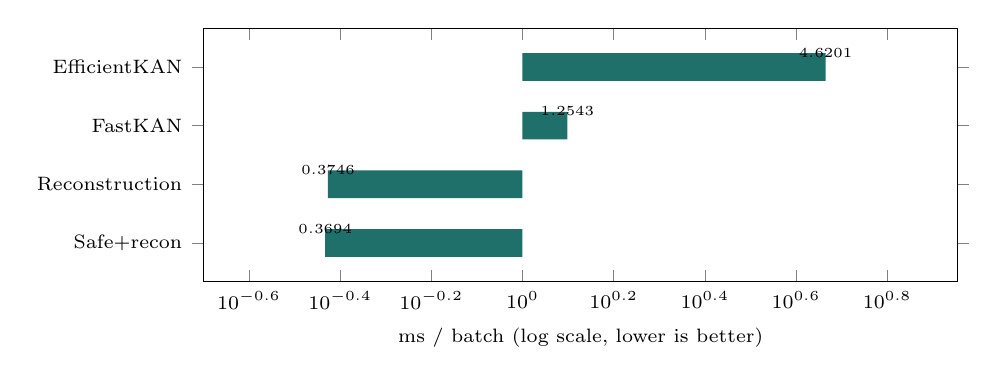
\begin{tikzpicture}
\begin{axis}[
  width=0.92\columnwidth, height=4.8cm,
  xbar, xmode=log,
  xlabel={ms / batch (log scale, lower is better)},
  xmin=0.2, xmax=9,
  symbolic y coords={Safe+recon,Reconstruction,FastKAN,EfficientKAN},
  ytick=data,
  tick label style={font=\scriptsize}, label style={font=\scriptsize},
  nodes near coords={\pgfmathprintnumber{\pgfplotspointmeta}},
  point meta=explicit,
  every node near coord/.append style={font=\tiny, /pgf/number format/.cd, fixed, precision=4},
  bar width=10pt, enlarge y limits=0.22,
]
\addplot[draw=none, fill=teal] coordinates {
  (0.3694,Safe+recon)[0.3694] (0.3746,Reconstruction)[0.3746]
  (1.2543,FastKAN)[1.2543] (4.6201,EfficientKAN)[4.6201]};
\end{axis}
\end{tikzpicture}
\caption{Per-batch plaintext latency on CIC-IDS2017 (log scale, mean over 5
seeds). Reconstruction variants are $3$--$12\times$ faster than FastKAN and
EfficientKAN.}
\label{fig:speed}
\end{figure}

\begin{figure}[t]
\centering
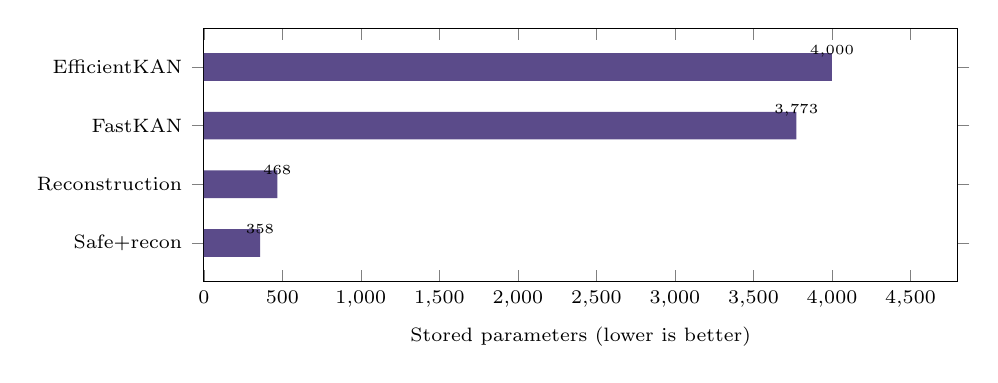
\begin{tikzpicture}
\begin{axis}[
  width=0.92\columnwidth, height=4.8cm,
  xbar,
  xlabel={Stored parameters (lower is better)},
  xmin=0, xmax=4800,
  symbolic y coords={Safe+recon,Reconstruction,FastKAN,EfficientKAN},
  ytick=data,
  tick label style={font=\scriptsize}, label style={font=\scriptsize},
  nodes near coords={\pgfmathprintnumber{\pgfplotspointmeta}},
  point meta=explicit,
  every node near coord/.append style={font=\tiny, /pgf/number format/.cd, fixed, precision=0},
  bar width=10pt, enlarge y limits=0.22,
]
\addplot[draw=none, fill=violet] coordinates {
  (358,Safe+recon)[358] (468,Reconstruction)[468]
  (3773,FastKAN)[3773] (4000,EfficientKAN)[4000]};
\end{axis}
\end{tikzpicture}
\caption{Stored parameters (mean over 5 seeds). Reconstruction is roughly
$8\times$ more compact than FastKAN and EfficientKAN; safe pruning reduces it
further to $358$.}
\label{fig:params}
\end{figure}

\subsection{Fidelity}

Because reconstruction reproduces the symbolic model's arithmetic exactly, its
predictions match the symbolic model to within floating-point rounding; the
mean per-sample logit deviation is $\approx 1.6\times10^{-4}$, effectively
zero. Safe pruning introduces a deliberately bounded change: by construction
each removed edge satisfies $\Delta\mathrm{AUC}\le\tau_{\mathrm{AUC}}$ and
$\Delta\mathrm{Acc}\le\tau_{\mathrm{Acc}}$, so the aggregate quality change
stays within the configured tolerance; on the real benchmark this corresponds
to a small AUC reduction ($0.9952\to0.9899$) in exchange for a smaller graph.
Reconstruction therefore preserves the symbolic model's predictions exactly,
while safe pruning offers a controlled accuracy-for-size trade.

\section{Discussion}

Two points are worth emphasising. First, reconstruction's predictions are
numerically identical to the symbolic model: its speed and compactness come
from collapsing the network into a fused polynomial, not from approximation, so
the efficiency gain carries no inherent accuracy cost. Second, the advantage
over FastKAN and EfficientKAN is specific to low-degree polynomial edges. When
each edge is a cheap polynomial, evaluating one fused expression per output is
faster than evaluating Gaussian basis functions per hidden unit (FastKAN) or
running a reparameterised spline (EfficientKAN), and it stores far fewer
parameters. For edges that are expensive to evaluate (for example high-order
splines), the gap would narrow; reconstruction is most advantageous precisely
when symbolification yields compact, low-degree expressions, the common case
after fitting a small symbolic library. We also note that FastKAN attains the
highest raw accuracy in our runs; reconstruction's contribution is efficiency
at comparable discrimination, not a new accuracy record.

Safe pruning is conservative by design. Its bounds guarantee that no removed
edge individually exceeds the tolerance, which is why it removes graph noise
without measurable degradation. It does not attempt aggressive compression; its
goal is a smaller \emph{exact} graph, not a smaller approximate one.

\section{Limitations}

The benchmark is single-machine; although we report mean\,$\pm$\,std over five
seeds, absolute latency is hardware-dependent. Safe pruning's ablation step is
computed on a validation set, so its guarantees are empirical rather than
analytical, and on real data it incurs a small accuracy reduction in exchange
for a smaller graph. The efficiency advantage over FastKAN and EfficientKAN is
contingent on low-degree symbolic edges and would narrow for expensive edge
functions. Finally, the study is restricted to plaintext inference; deployment
under encrypted inference is a separate concern and is not measured here.

\section{Conclusion}

Symbolifying a KAN makes it interpretable but not fast, because framework
overhead dominates inference. Exact symbolic reconstruction removes that
overhead by evaluating the closed-form expression graph directly, with
predictions numerically identical to the symbolic model. On a multi-seed
CIC-IDS2017 benchmark, reconstruction runs $3.4\times$ faster than FastKAN and
$12.3\times$ faster than EfficientKAN while using roughly $8\times$ fewer
parameters, at comparable discrimination; safe pruning shrinks the graph
further under explicit ablation bounds. Reconstruction is a simple, drop-in
accelerator for any trained symbolic KAN.

\begin{thebibliography}{00}

\bibitem{kan}
Z. Liu et al., ``KAN: Kolmogorov--Arnold Networks,''
\emph{arXiv preprint arXiv:2404.19756}, 2024.

\bibitem{cicids}
I. Sharafaldin, A. H. Lashkari, and A. A. Ghorbani,
``Toward Generating a New Intrusion Detection Dataset and Intrusion Traffic
Characterization,'' in \emph{Proc. ICISSP}, 2018.

\bibitem{fastkan}
Z. Li, ``FastKAN: Very Fast Implementation of Kolmogorov--Arnold Networks
with Gaussian Radial Basis Functions,'' 2024, software.
\url{https://github.com/ZiyaoLi/fast-kan}.

\bibitem{effkan}
Blealtan, ``Efficient-KAN: An Efficient Implementation of Kolmogorov--Arnold
Networks,'' 2024, software.
\url{https://github.com/Blealtan/efficient-kan}.

\end{thebibliography}

\end{document}
